\chapter{Specific Requirements}

\begin{justify}
    This section details all the specific requirements of the PeerFlow system. These requirements describe the functionalities and non-functional attributes that the system must possess. They are categorized to provide clarity and ensure completeness, serving as the foundation for the design, development, and testing phases of the project. Each requirement should be clear, unambiguous, verifiable, and traceable.
\end{justify}


\section{Functional Requirements}

\begin{justify}
   This subsection outlines the specific functionalities that PeerFlow must provide to its users (teachers and students). Each functional requirement describes an action that the system must perform, how it should react to specific inputs, or what it should allow users to do. These requirements will often be further detailed with use cases, user stories, or detailed input/output descriptions in subsequent sections or annexes. Functional requirements are prioritized using "MoSCoW Prioritization":
   \begin{itemize}
       \item \textbf{M - Must have}: Non-negotiable product needs that are mandatory for the team.
       \item \textbf{S - Should have}: Important initiatives that are not vital, but add significant value.
       \item  \textbf{C - Could Have}: Nice to have initiatives that will have a small impact if left out.
       \item \textbf{W - Will not have}: Initiatives that are not a priority for this specific time frame.
   \end{itemize}
\end{justify}

\begin{justify}
    For a better understanding of the system's operations, each subsection within the subsequent "Functional Requirements" section will be accompanied by a concise activity diagram to visually clarify the main activity flow of the described requirements.
\end{justify}

\clearpage

\vspace*{1cm}

\subsection{General System}

\begin{table}[h]
    \centering
    \begin{tabular}{|l|c|p{10cm}|}
        \hline
        \textbf{ID} & \textbf{Priority} & \textbf{Requirement} \\
        \hline
        FR-SYS-001 & M & The system shall support two distinct user roles: Teacher and Student. \\
        \hline
        FR-SYS-002 & M & The system shall require users to authenticate before accessing role-specific functionalities. \\
        \quad FR-SYS-002.UI &  & \quad The system's UI shall present a typical login page (email and password) as the initial point of interaction for unauthenticated users attempting to access the system. \\
        \quad FR-SYS-002.BL &  & \quad The system's BL shall validate submitted user credentials (handling the invalid credential case), identify the authenticated user's pre-assigned role and enforce access restrictions by granting access only to the system functionalities, data, and user interface views appropriate for the identified user role. \\
        \hline
        FR-SYS-003 & M & The system shall allow new users (Students or Teachers) to sign up. \\
        \quad FR-SYS-003.UI &  & \quad The system’s UI shall provide a clearly identifiable link or button (e.g., labeled "Sign Up" or "Register") on the login page, which navigates the user to a dedicated registration page. The Sign Up Page should select if the user is a Student or a Teacher and insert name, surname, email (unique) and password, with a Sign Up button to confirm. \\
        \quad FR-SYS-003.BL &  & \quad The system’s BL, should validate (check if a user with the same email already exists) and register the new user. \\
        \hline
    \end{tabular}
    \caption{General System Functional Requirements.}
    \label{tab:GeneralSystemFR}
\end{table}

\clearpage
\vspace*{\fill}
\begin{figure}[h]
    \centering
    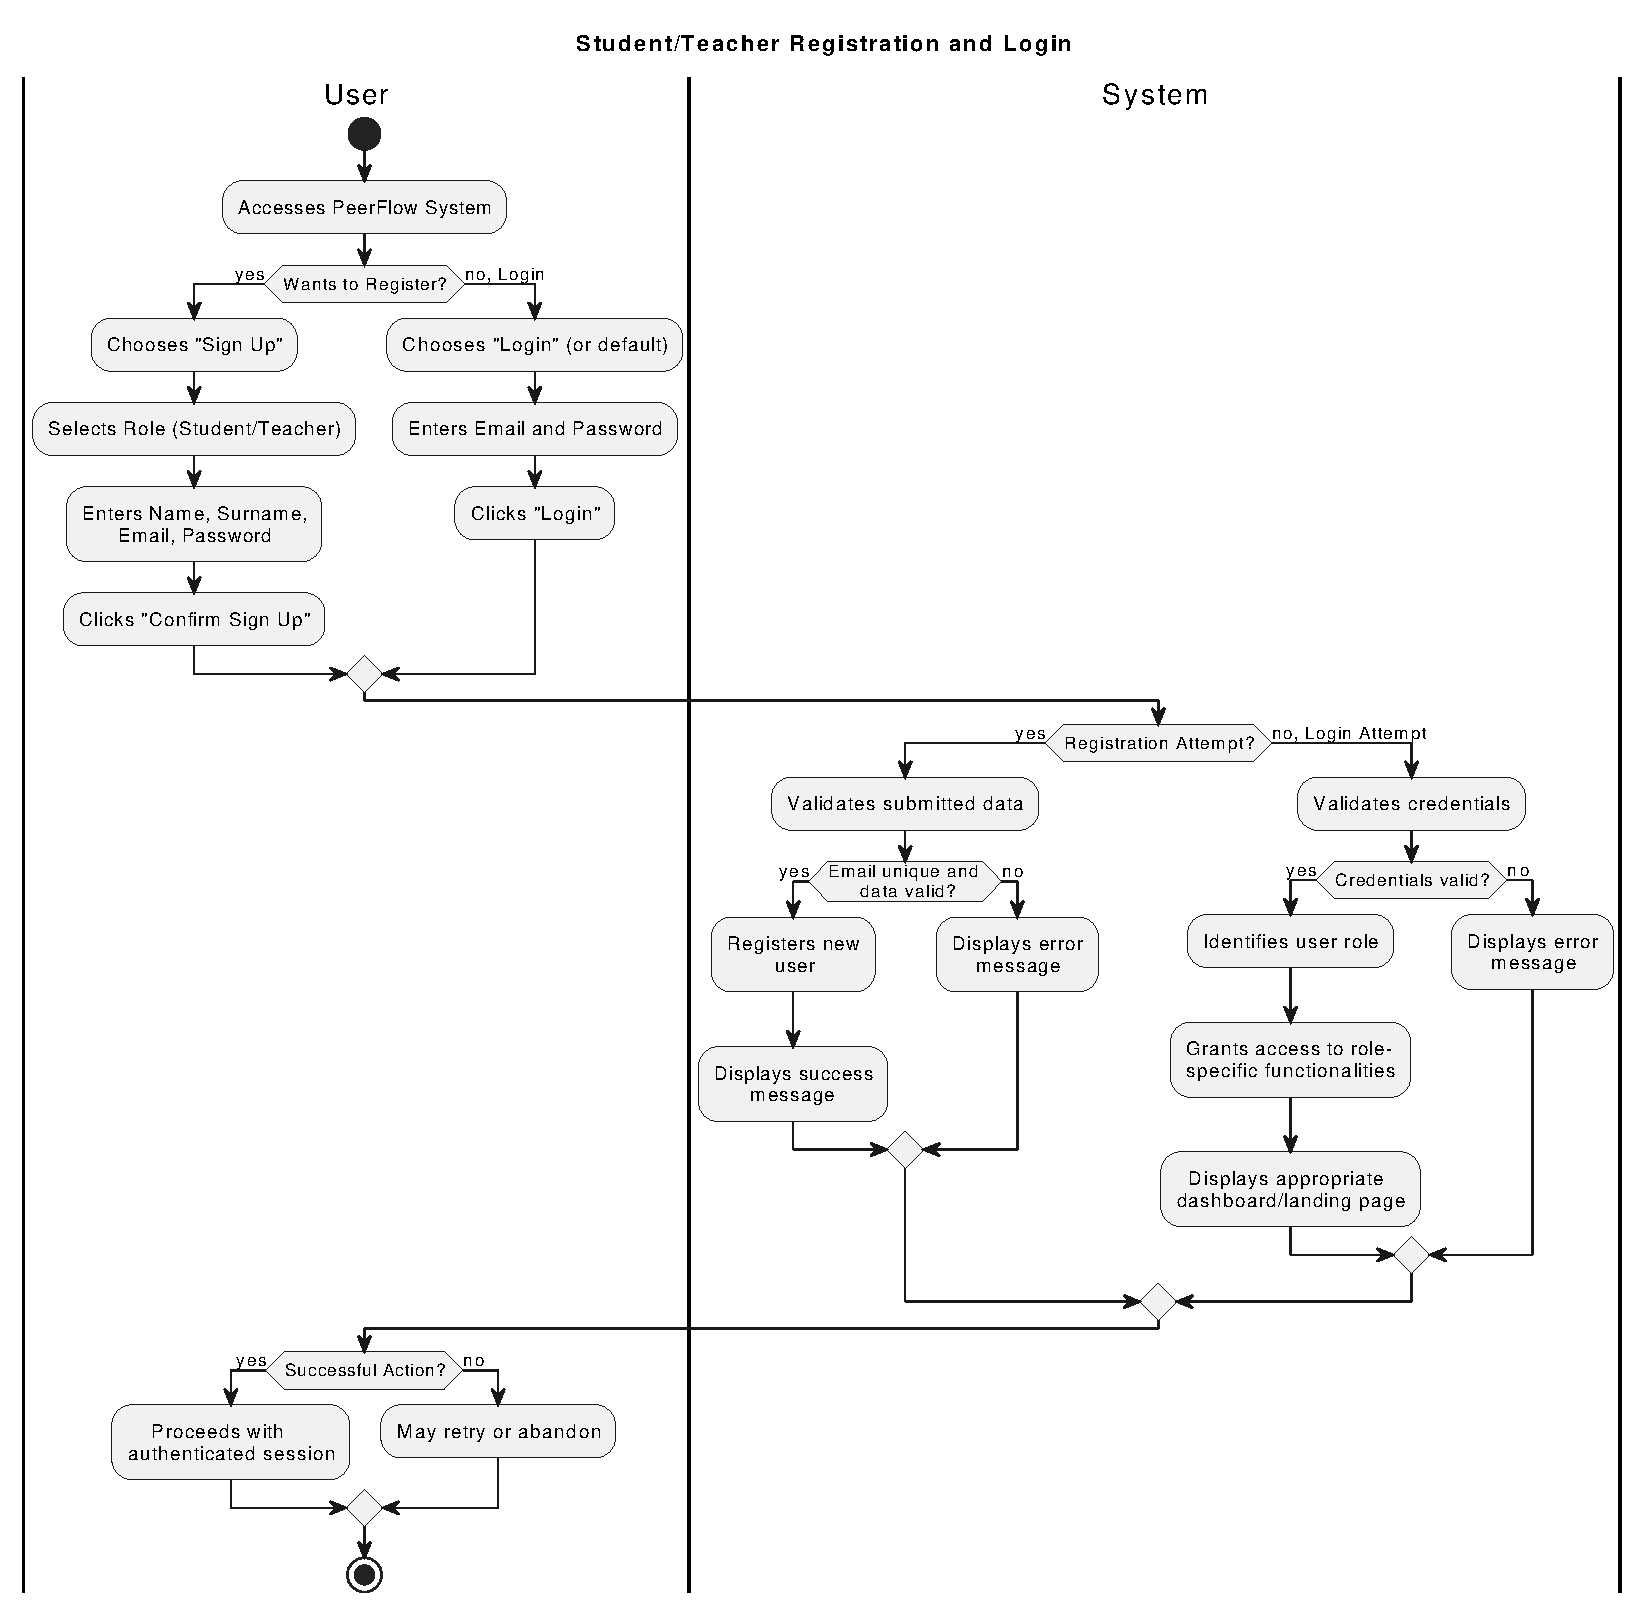
\includegraphics[width=1\linewidth]{SRS/imgs/1_GeneralSystemAD.pdf}
    \caption{General System Student/Teacher Registration and Login Activity Diagram.}
    \label{fig:GeneralSystemAC}
\end{figure}
\vspace*{\fill}

\clearpage

\vspace*{-1cm}

\subsection{Assignment Management - Teacher}

    \begin{tabular}{|l|c|p{10cm}|}
        \hline
        \textbf{ID} & \textbf{Priority} & \textbf{Requirement} \\
        \hline
        FR-ASG-001 & M & The system shall enable authenticated Teachers to view a list of all assignments within the system. \\
        \quad FR-ASG-001.UI &  & \quad The system's UI shall provide a dedicated section or page, accessible to authenticated Teachers, specifically for displaying assignments (for each show name, status [assigned, preparing review, under review, completed, deleted], and last modified date). The UI shall provide a mechanism to navigate from an assignment in the list to a more detailed view or management page for that specific assignment (name, description, deadline, current status, list of students involved, created data). \\
        \quad FR-ASG-001.BL &  & \quad The system’s BL shall provide the list of created assignments for the specific authenticated Teacher. In case of navigate into the detailed page of an assignment, the BL shall retrieve the necessary data fields (name, description, deadline, current status, list of students involved, created data). \\
        \hline
        FR-ASG-002 & M & The system shall allow authenticated Teachers to create new assignments. \\
        \quad FR-ASG-002.UI &  & \quad The system's UI shall provide a mechanism for authenticated Teachers to initiate the creation of a new assignment (e.g., a "Create New Assignment" button or link accessible from assignments list page). Upon initiating assignment creation, the UI shall present a form or dedicated page where the Teacher can input the details for the new assignment (name, description, deadline, list of students involved). The UI shall provide a button (e.g., "Create Assignment," "Save Assignment") to submit the new assignment details. \\
        \quad FR-ASG-002.BL &  & \quad Upon submission of the new assignment creation form by an authenticated Teacher, the system's business logic shall validate the fields (check the deadline is in the future), generate a new assignment record in the data store and storing all provided details (Title, Description, Deadline, list of involved Student IDs, and add the Assignment to the appropriate list of the students involved). \\
        \hline
    \end{tabular}

\begin{table}[h]
    \centering
    \caption{Teacher Assignment Management Functional Requirements (1-2).}
    \label{tab:AssignmentManagerTeacherFR1}
\end{table}

\clearpage
\vspace*{\fill}
\begin{table}[h]
    \centering
    \begin{tabular}{|l|c|p{10cm}|}
        \hline
        \textbf{ID} & \textbf{Priority} & \textbf{Requirement} \\
        \hline
        FR-ASG-003 & S & The system shall enable authenticated Teachers to modify the details of assignments, provided the modification attempt occurs before the assignment's current submission deadline has passed. Modifiable details include the assignment title, description, submission deadline, and the list of involved students. \\
        \quad FR-ASG-003.UI &  & \quad From an assignment's detail view page, if the assignment's current submission deadline has not yet passed, the system's UI shall present a clearly identifiable "Edit Assignment" button or link to authenticated Teachers who created the assignment. This option shall be absent or disabled if the deadline has passed. The editing interface shall be pre-populated with the current details of the assignment being edited. \\
        \quad FR-ASG-003.BL &  & \quad The business logic shall verify that the assignment's original submission deadline (the deadline stored before this modification attempt) has not yet passed. If it has passed, the modification shall be rejected or not shown. The business logic shall validate all submitted modified fields. \\
        \hline
    \end{tabular}
    \caption{Teacher Assignment Management Functional Requirements (3).}
    \label{tab:AssignmentManagerTeacherFR2}
\end{table}


\vspace*{\fill}

\clearpage

\vspace*{\fill}
\begin{table}[h]
    \centering
   \begin{tabular}{|l|c|p{10cm}|}
        \hline
        \textbf{ID} & \textbf{Priority} & \textbf{Requirement} \\
        \hline
        FR-ASG-004 & S & The system shall enable authenticated Teachers to soft delete assignments (change its state to “deleted”), provided that the assignment's peer review process has not been finalized and results have yet been aggregated and made available to students. \\
        \quad FR-ASG-004.UI &  & \quad The system's UI shall provide a "Delete Assignment" button or link for assignments listed in the Teacher's assignment overview or/and on an assignment's detail page. This "Delete Assignment" option shall only be visible and enabled for assignments created by the authenticated Teacher and for which the peer review process has not been finalized and results are not yet available. Upon initiating the deletion action, the UI shall present a confirmation dialog to the Teacher. The assignment shall remain in the list of teacher’s and student’s assignments, but with the “deleted” status (all the button disappear). \\
        \quad FR-ASG-004.BL &  & \quad The system's business logic shall first verify that the authenticated Teacher, then check the current status of the assignment to determine if it is eligible for deletion (results of the peer review phase have been made available to students). If the assignment is eligible for the deletion, the BL shall change the assignment status to “deleted”. All the other operation for that assignment are disabled. \\
        \hline
        FR-ASG-005 & C & The system shall notify involved students (through email) when a new assignment is created, (soft) deleted or an existing one is significantly updated (description or deadline). \\
        \hline
    \end{tabular}
    \caption{Teacher Assignment Management Functional Requirements (4-5).}
    \label{tab:AssignmentManagerTeacherFR3}
\end{table}

\vspace*{\fill}

\begin{figure}[h]
    \centering
    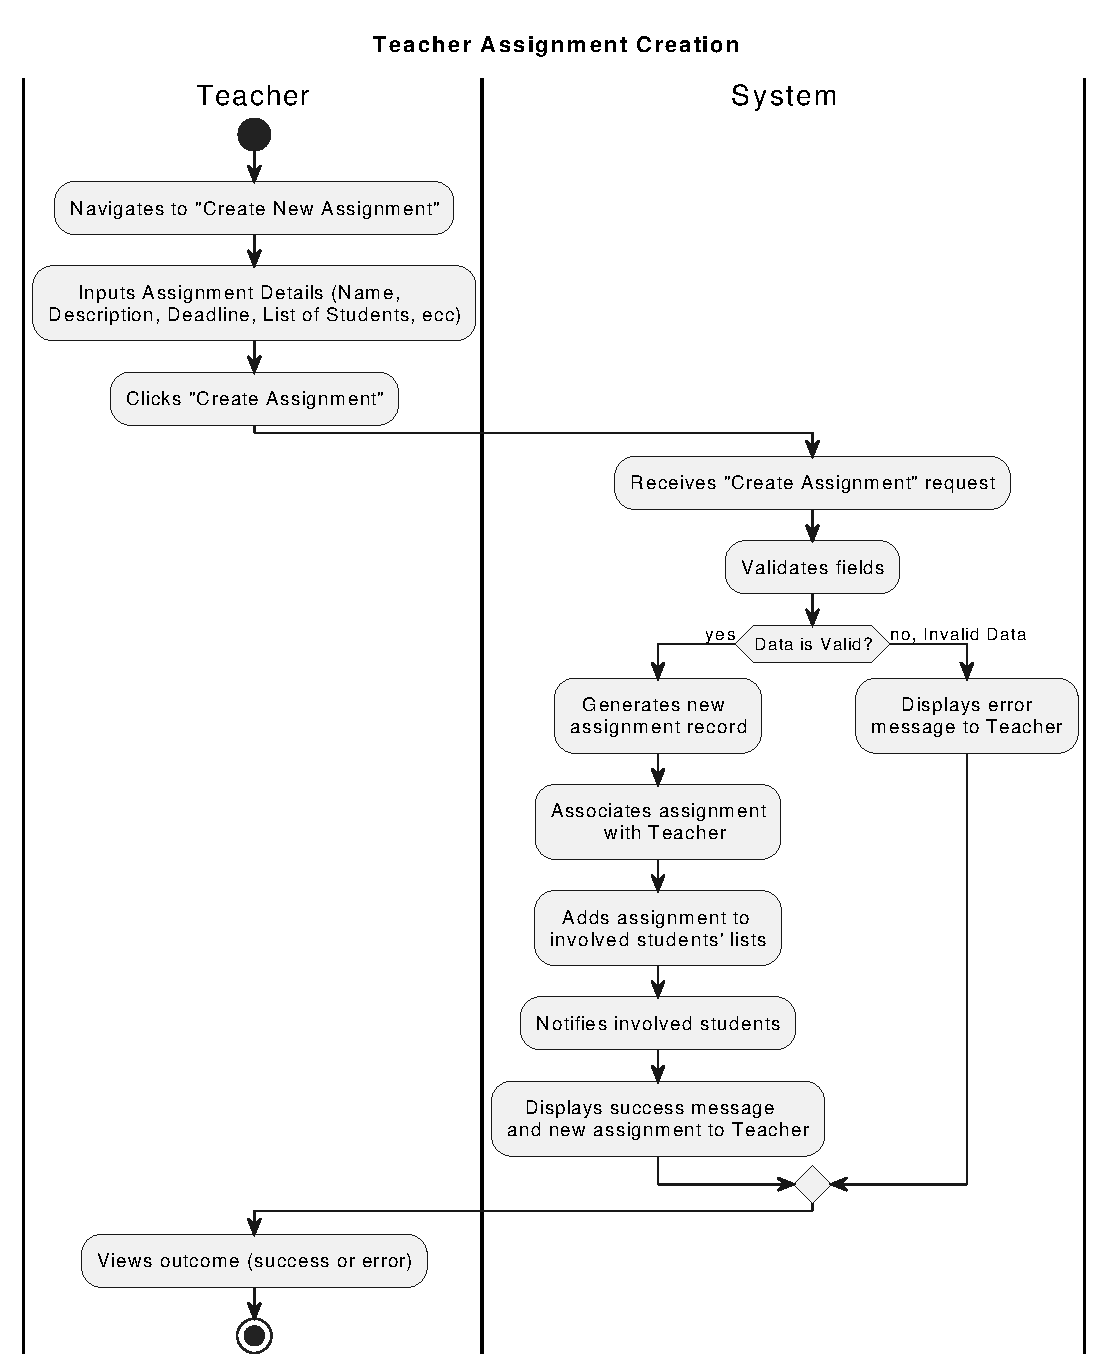
\includegraphics[width=1\linewidth]{SRS/imgs/2_TeacherManagementAD.pdf}
    \caption{Teacher Assignment Creation Activity Diagram.}
    \label{fig:TeacherAssignmentCreationAD}
\end{figure}
\vspace*{\fill}

\clearpage
\vspace*{\fill}

\subsection{Assignment Management - Student}

\begin{table}[h]
    \centering
    \begin{tabular}{|l|c|p{10cm}|}
        \hline
        \textbf{ID} & \textbf{Priority} & \textbf{Requirement} \\
        \hline
        FR-ASG-006 & M & The system shall allow authenticated Students to view the list of assignments they are involved in. \\
        \quad FR-ASG-006.UI &  & \quad The system's UI shall provide a dedicated section or page, accessible to authenticated Students, specifically for displaying assignments they are involved in (for each show name, status, and last modified date). The UI shall provide a mechanism to navigate from an assignment in the list to a more detailed view or management page for that specific assignment (name, description, deadline, current status, list of students involved, created data). \\
        \quad FR-ASG-006.BL &  & \quad The system’s BL shall provide the list of assignments for the specific authenticated Student. In case of navigate into the detailed page of an assignment, the BL shall retrieve the necessary data fields (name, description, deadline, current status, list of students involved, created data). \\
        \hline
    \end{tabular}
    \caption{Student Assignment List View Functional Requirements.}
    \label{tab:StudentAssignmentViewFR}
\end{table}
\vspace*{\fill}

\clearpage
\vspace*{\fill}
\subsection{Submission - Student}

\begin{table}[h]
    \centering
    \begin{tabular}{|l|c|p{10cm}|}
        \hline
        \textbf{ID} & \textbf{Priority} & \textbf{Requirement} \\
        \hline
        FR-SUB-001 & M & The system shall enable authenticated Students, who are involved in a specific assignment, to submit their work for that assignment before its submission deadline. Submissions shall consist of textual input and may optionally include file attachments of specified types. \\
        \quad FR-SUB-001.UI &  & \quad From an assignment's detail view page, if the current date/time is before the assignment's submission deadline and the authenticated Student has not yet submitted their work the system's UI shall present a clearly identifiable "Submit Work" or "Upload Submission" button/link. This option shall be absent or disabled otherwise. Activating the "Submit Work" option shall navigate the Student to a dedicated submission page/modal for that assignment, where he can submit a text, and the possibilities of upload a file (PDF, TXT o JPG). After submit with a button, the UI shall return to the details page of the assignment with the submission shown. \\
        \quad FR-SUB-001.BL &  & \quad The BL, shall verify that the current system date/time is before the assignment's official submission deadline. If possible should validate the input and register text (mandatory), attachments (if present), timestamp of submission. If all verifications and validations pass the system shall store all the input, the date timestamp and mark this assignment as “submitted” for the student. \\
        \hline
        FR-SUB-002 & M & The system shall allow students to view/download their own submitted work in the detailed assignment page. \\
        \hline
    \end{tabular}
    \caption{Student Assignment Submission Functional Requirements (1-2).}
    \label{tab:StudentAssignmentSubmissionFR}
\end{table}

\vspace*{\fill}
\clearpage
\vspace*{\fill}

\begin{table}[h]
    \centering
    \begin{tabular}{|l|c|p{10cm}|}
        \hline
        \textbf{ID} & \textbf{Priority} & \textbf{Requirement} \\
        \hline
        FR-SUB-003 & S & The system shall enable authenticated Students, who are involved in a specific assignment, to edit all the part of their submitted work for that assignment before its submission deadline. Submissions shall consist of textual input and may optionally include file attachments of specified types. \\
        \quad FR-SUB-003.UI &  & \quad From an assignment's detail view page, if the current date/time is before the assignment's submission deadline and the authenticated Student has submitted their work the system's UI shall present a clearly identifiable "Edit Work" or "Edit Submission" button/link. This option shall be absent or disabled otherwise. Activating the "Edit Work" option shall navigate the Student to the same page/modal described in the FR-SUB-001.UI for that assignment, with the field filled with their upload, with the possibilities to edit everything. After submit with a button, the UI shall return to the details page of the assignment with the new submission shown. \\
        \quad FR-SUB-003.BL &  & \quad The BL, shall verify that the current system date/time is before the assignment's official submission deadline. If possible, shall retrieve the previous submission to fill the fields, and should validate, if edited, the input and register text (mandatory), attachments (if present), and update the timestamp of submission. If all verifications and validations pass the system shall store all the input. If all the fields are empty, the BL shall remove the “submitted” mark for the student. \\
        \hline
    \end{tabular}
    \caption{Student Assignment Submission Functional Requirements (3).}
    \label{tab:StudentAssignmentSubmissionFR2}
\end{table}

\begin{figure}[h]
    \centering
    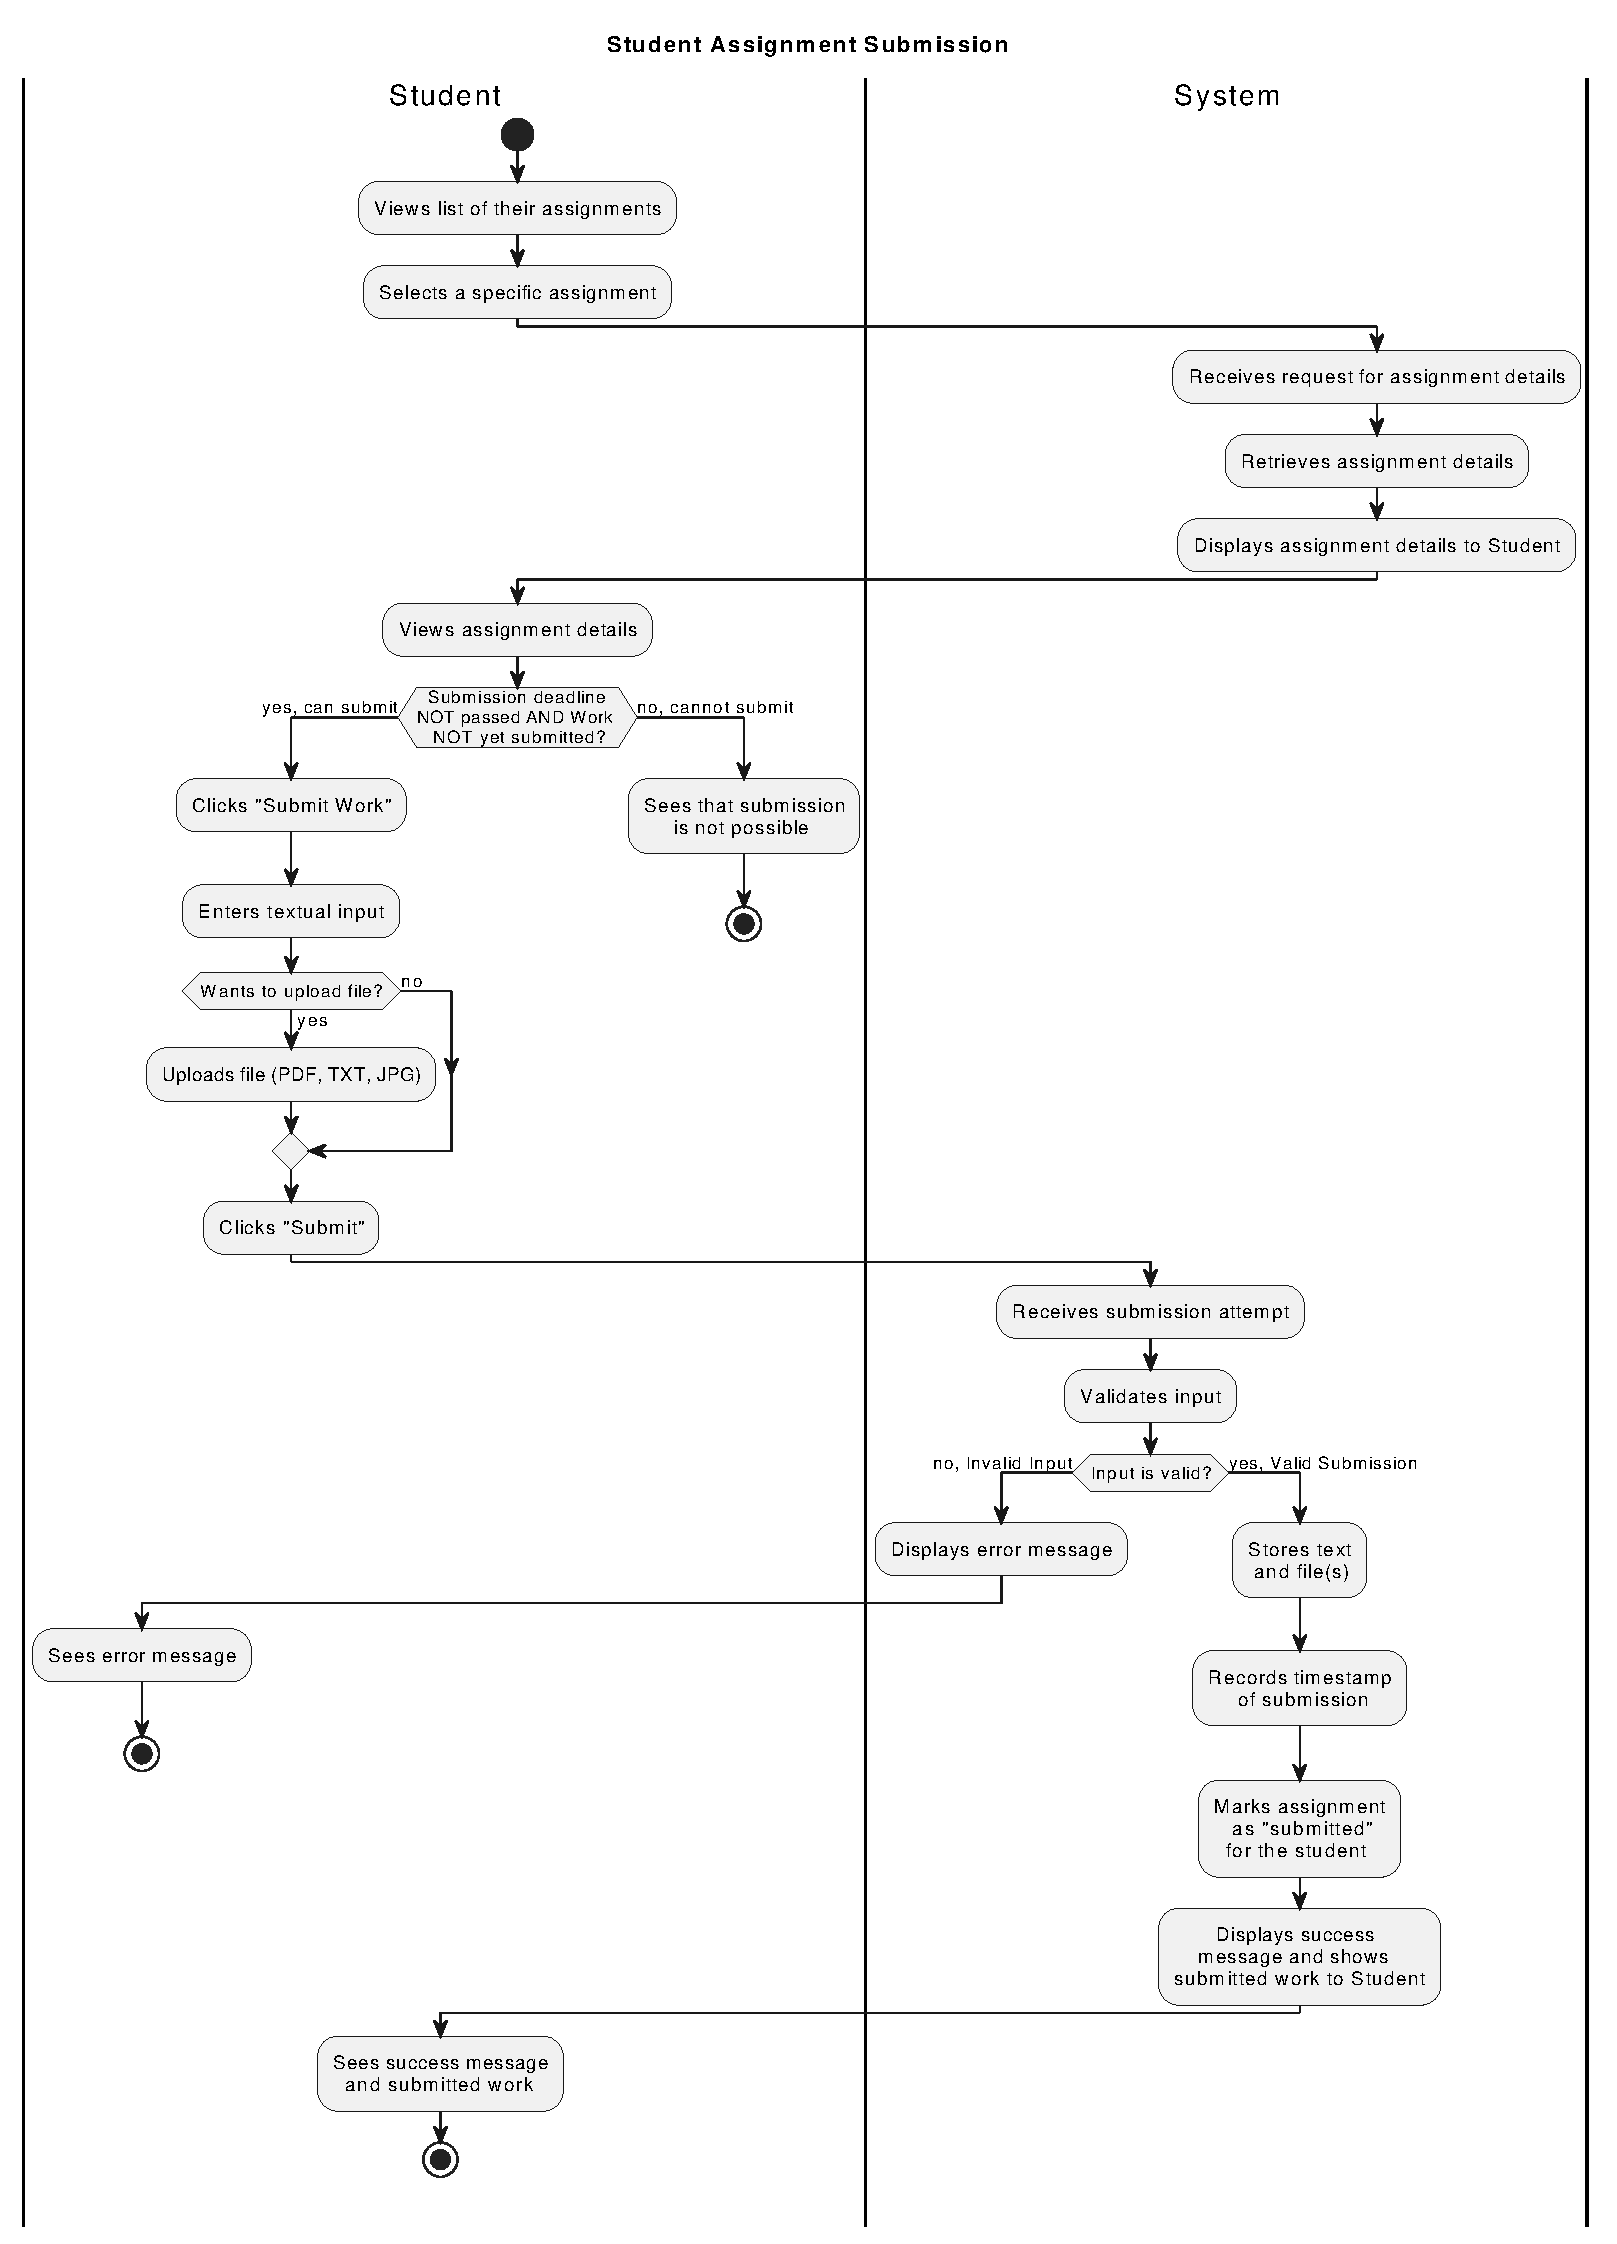
\includegraphics[width=1\linewidth]{SRS/imgs/3_StudentSubmissionAD.pdf}
    \caption{Student Assignment Submission Activity Diagram.}
    \label{fig:StudentAssignmentAD}
\end{figure}
\vspace*{\fill}
\clearpage

\vspace*{\fill}
\subsection{Peer Review Assignment - Teacher}
    \begin{tabular}{|l|c|p{10cm}|}
         \hline
        \textbf{ID} & \textbf{Priority} & \textbf{Requirement} \\
        \hline
        FR-PRV-001 & S & The system shall enable authenticated Teachers to define and associate a new assessment rubric with a specific assignment, only after the assignment's submission deadline has passed and provided a rubric has not already been finalized for it. A rubric shall consist of one or more criteria, each with a title, a detailed description, and a defined scoring range (e.g., 0 to 5 points). \\
        \quad FR-PRV-001.UI &  & \quad On an assignment's detail view page, if the assignment's submission deadline has passed and no rubric has yet been finalized for it, the system's UI shall present a clearly identifiable "Define Rubric" or "Set Evaluation Rubric" button/link to the authenticated Teacher. Activating this option shall navigate the Teacher to a rubric creation interface specifically for that assignment. The rubric creation interface shall allow the Teacher to define one or more evaluation criteria. For each criterion, input: title description, scoring range (define a minimum and maximum numerical score range (e.g., Min: 0, Max: 5)). Provide an option to remove criteria during the definition process. The UI shall provide a button (e.g., "Save Rubric," "Finalize Rubric") to submit the defined rubric for the assignment. A "Cancel" button shall also be provided. Upon successful creation and association of the rubric, the UI shall provide clear visual feedback (e.g., a success message) and display the defined rubric on the assignment's detail page. \\
        \quad FR-PRV-001.BL &  & \quad The BL shall verify that the submission deadline for the target assignment has indeed passed. The BL shall verify that a rubric has not already been finalized and associated with this assignment. The BL shall validate the submitted rubric data: at least one criterion must be defined; for each criterion, a Title, Description, and a valid Scoring Range (e.g., min score <= max score, non-negative integers) must be provided. If all verifications and validations pass, the system shall create a new rubric record in the data store, including all its criteria, and associate this newly created rubric with the target assignment. \\
        \hline
    \end{tabular}
\begin{table}[h]
    \centering
    \caption{Teacher Peer Review Creation Functional Requirements (1).}
    \label{tab:TeacherPeerReviewFR1}
\end{table}
\vspace*{\fill}
\clearpage
\vspace*{\fill}
\begin{table}[h]
    \centering
    \begin{tabular}{|l|c|p{10cm}|}
        \hline
        \textbf{ID} & \textbf{Priority} & \textbf{Requirement} \\
        \hline
        FR-PRV-002 & S & The system shall enable authenticated Teachers to edit the defined assessment rubric with a specific assignment they have created. \\
        \quad FR-PRV-002.UI &  & \quad On an assignment's detail view page, near the defined rubrics, the system's UI shall present a clearly identifiable “Edit Rubric" button/link to the authenticated Teacher. Activating this option shall navigate the Teacher to the rubric creation interface populated with the defined data during the creation. The UI shall provide a button (e.g., "Save Rubric," "Finalize Rubric") to submit the edited rubric for the assignment. A "Cancel" button shall also be provided in order to cancel the update done. \\
        \quad FR-PRV-002.BL &  & \quad The BL shall verify that a rubric exists. The BL shall retrieve the defined rubrics data to populate the fields. The BL shall validate the submitted rubric data: at least one criterion must be defined; for each criterion, a Title, Description, and a valid Scoring Range (e.g., min score <= max score, non-negative integers) must be provided. If all verifications and validations pass, the system shall update the rubric record in the data store, including all its criteria. \\
        \hline
        FR-PRV-003 & S & The system shall enable authenticated Teachers to delete the defined assessment rubric with a specific assignment. \\
        \quad FR-PRV-003.UI &  & \quad On an assignment's detail view page, near the defined rubrics, the system's UI shall present a clearly identifiable “Delete Rubric" button/link to the authenticated Teacher who created the assignment and rubric. Activating this option shall remove the created rubric. \\
        \quad FR-PRV-003.BL &  & \quad The BL shall verify that a rubric exists. The BL shall delete the rubrics associated with the assignment. \\
        \hline
    \end{tabular}
    \caption{Teacher Peer Review Creation Functional Requirements (2-3).}
    \label{tab:TeacherPeerReviewFR2}
\end{table}
\vspace*{\fill}

\clearpage

\begin{longtable}{|l|c|p{10cm}|}
    \hline
    \textbf{ID} & \textbf{Priority} & \textbf{Requirement} \\
    \hline
    FR-PRV-004 & M & The system shall enable authenticated Teachers to configure and initiate the peer review process for a specific course assignment they manage. This configuration shall occur after student submissions for the assignment have closed and an evaluation rubric has been finalized (as per FR-PRV-001). Configuration options shall include setting the number of peer reviewers per submission, confirming the finalized rubric (create one if not present), and choosing between automatic or manual reviewer assignment. The system must prevent any student from being assigned their own submission to review. Once initiated, the peer review phase can only be halted by the Teacher deleting the entire assignment; no other mechanism to stop or pause the review phase for an individual assignment will be provided. \\
    \quad FR-PRV-004.UI &  & \quad On an assignment's detail view page, if student submissions have closed (and peer review has not yet been initiated), the system's UI shall present a "Setup Peer Review" or "Configure Reviewers" button/link to the authenticated Teacher. Activating this option shall navigate the Teacher to a dedicated peer review configuration interface for that assignment. This interface shall display: a read-only view or summary of the finalized rubric for confirmation (if created, instead the “Create Rubric” button shall be shown); an input field for "Number of Reviewers per Submission" (numerical input); a selection mechanism for "Reviewer Assignment Mode" with options: "Automatic" and "Manual." If "Automatic" assignment mode is selected, no further student selection UI is immediately required on this initial setup screen. If "Manual" assignment mode is selected, the UI shall additionally present: a list of students who have submitted work for this assignment. For each submitting student (or their submission), a mechanism to select the specified number of unique peer reviewers from the pool of other students who have also submitted work for this assignment. The UI must prevent the selection of a student to review their own submission. The interface shall include a button (e.g., "Start Peer Review," "Initiate Reviews"). 
   \hline
\end{longtable}

\begin{table}[h]
    \centering
    \caption{Teacher Peer Review Creation Functional Requirements (4).}
    \label{tab:TeacherPeerReviewFR4}
\end{table}

\clearpage
\begin{longtable}{|l|c|p{10cm}|}
    \hline
    \textbf{ID} & \textbf{Priority} & \textbf{Requirement} \\
    \hline
     &  & (e.g., The UI shall provide clear visual feedback upon successful initiation of the peer review phase (e.g., a success message, assignment status update) or indicate specific input errors if initiation fails "Number of reviewers must be at least 1," "Not enough eligible reviewers for automatic assignment," "All submissions must have the required number of manual reviewers assigned," "Rubric not confirmed"). Once the peer review phase is initiated for an assignment, the "Setup Peer Review" option shall no longer be available for that assignment. UI elements related to modifying the review configuration (other than deleting the entire assignment) shall be absent or disabled. \\
    \quad FR-PRV-004.BL &  & \quad Upon a Teacher's request to initiate the peer review phase for an assignment, the system's BL shall verify: the authenticated Teacher, the assignment's submission deadline has passed, and submissions are closed, the peer review phase has not already been initiated for this assignment. The BL shall validate the provided configuration parameters. The system shall then automatically assign the specified number of unique peer reviewers to each submission, ensuring no student is assigned their own submission. The system shall create the necessary peer review pairing records in the data store (linking reviewer, reviewee's submission, and the assignment). The system shall update the status of the assignment to "Peer Review in Progress." The system shall make the assigned submissions and the confirmed rubric available to the assigned student reviewers. If any verification or validation fails, the system shall prevent the initiation of the peer review phase and provide appropriate error information to be surfaced by the UI. Once an assignment's status is "Peer Review in Progress," the business logic shall prevent any further modifications to its peer review configuration (number of reviewers, assignment mode, pairings) or rubric. The only way to alter this state via Teacher action is through assignment deletion. \\
    \hline
    FR-PRV-005 & S & The system shall notify students on email when they have been assigned peer reviews. \\
    \hline
\end{longtable}
\begin{table}[h]
    \centering
    \caption{Teacher Peer Review Creation Functional Requirements (4-5).}
    \label{tab:TeacherPeerReviewFR5}
\end{table}

\vspace*{\fill}
\begin{figure}[h]
    \centering
    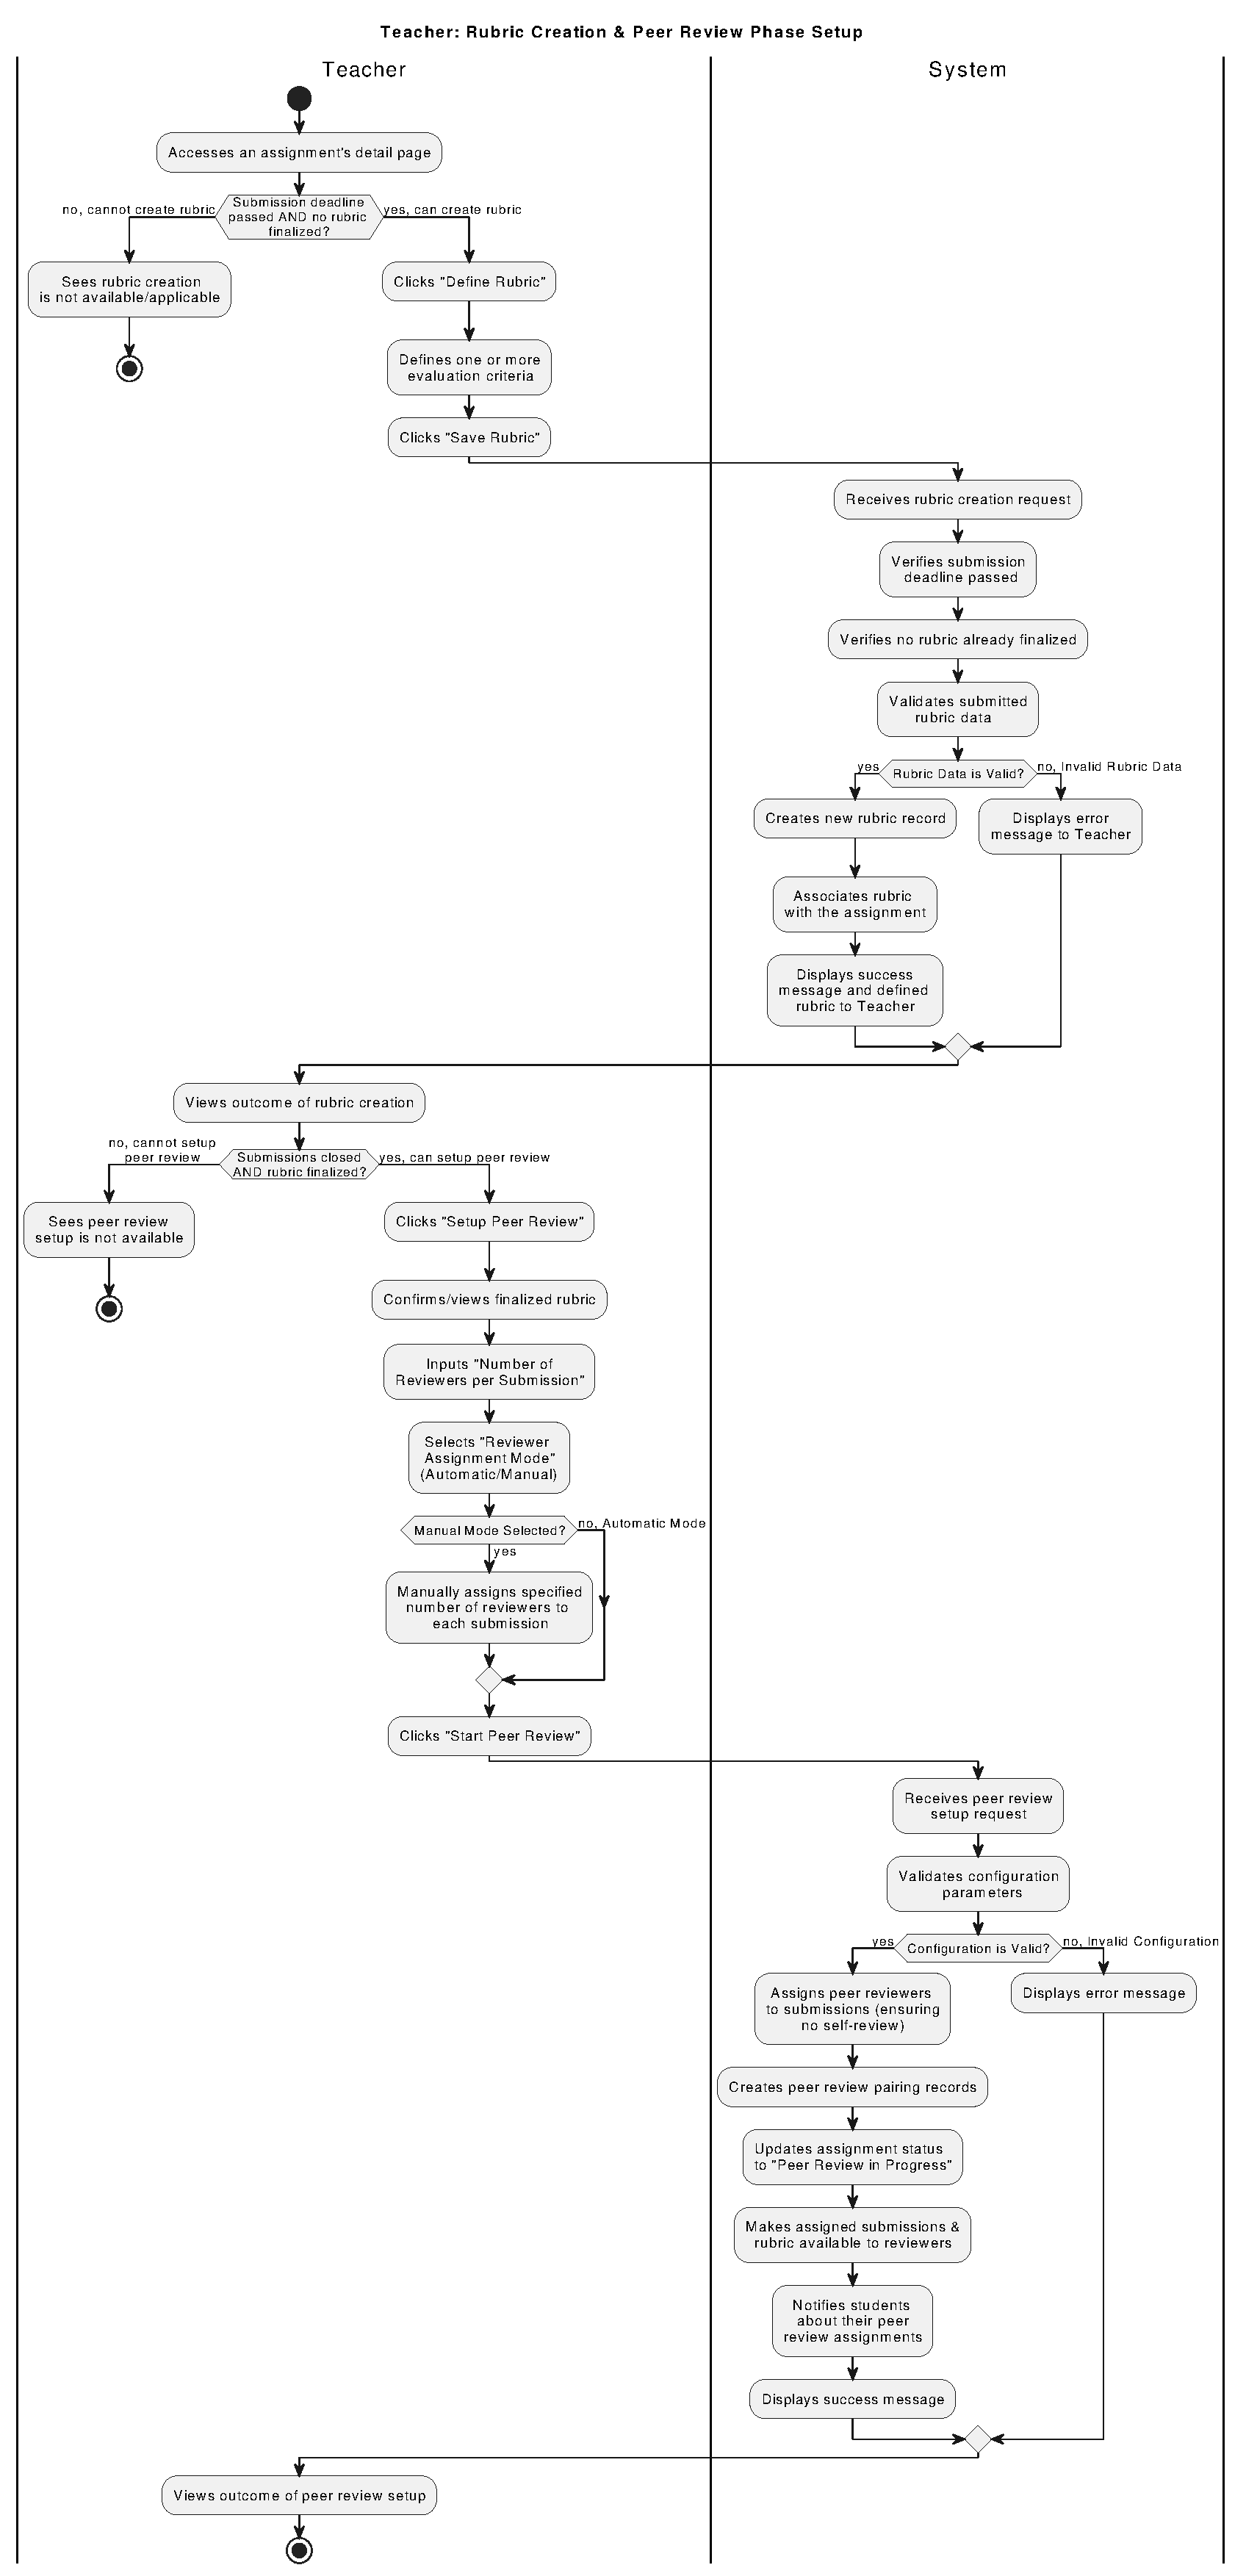
\includegraphics[width=.7\linewidth]{SRS/imgs/4_TeacherPeerCreation.pdf}
    \caption{Teacher Peer Review Creation Activity Diagram.}
    \label{fig:TeacherPeerReviewCreationAD}
\end{figure}
\vspace*{\fill}
\clearpage

\subsection{Reviewing - Student}
    
    \begin{tabular}{|l|c|p{10cm}|}
        \hline
        \textbf{ID} & \textbf{Priority} & \textbf{Requirement} \\
        \hline
        FR-REV-001 & M & The system shall enable authenticated Students to access and view the specific assignment submissions that have been allocated to them for peer review, along with the associated evaluation rubric, once an assignment has entered the peer review stage. \\
        \quad FR-REV-001.UI &  & \quad When an assignment is in the "Peer Review" stage, the system's UI shall present to an authenticated Student a dedicated section or page listing all submissions currently assigned to them for review for that specific assignment, including for each submission an identifier (the submitting student’s name must not be visible), the title, the deadline and the status of the review (“In progress”, “Completed”). The UI shall provide a button to view/access the evaluation Rubric associated with the parent assignment from the list view. From the list of assigned submissions, the Student shall be able to select an individual submission to open a detailed review interface for that specific submission, including the submitted text content and a list of any attached files, allowing the Student to view or download them. \\
        \quad FR-REV-001.BL &  & \quad When an authenticated Student requests to view submissions assigned to them for review for a specific assignment that is in the "Peer Review" stage the business logic shall query the data store to identify all submission records specifically allocated to this Student for review within that assignment, and for each allocated submission retrieve the necessary data for display as specified in the FR-REV-001.UI. The business logic shall retrieve the evaluation Rubric associated with the parent assignment when required. When the Student requests to view a single assignment, the business logic shall retrieve the content of the assignment (text and file attachments). \\
        \hline
        FR-REV-ANON-001 & M & For each submission assigned to a student for peer review of a specific assignment, any personally identifiable information (PII) of the submitter must be concealed from the reviewer. \\
        \hline
    \end{tabular}
\begin{table}[h]
    \centering
    \caption{Student Reviewing Functional Requirements (1).}
    \label{tab:StudentReviewingFR1}
\end{table}

\begin{table}[h]
    \centering
    \begin{tabular}{|l|c|p{10cm}|}
        \hline
        \textbf{ID} & \textbf{Priority} & \textbf{Requirement} \\
        \hline
        FR-REV-002 & M & The system shall enable authenticated Students to conduct and submit a peer review for an assigned submission, requiring them to provide a score (within the rubric's defined range) and a textual justification for each criterion in the associated evaluation rubric. Submission of the review shall only be possible once all required criteria are addressed. \\
        \quad FR-REV-002.UI &  & \quad Within the detailed review interface for a single submission the system's UI shall provide a button for the Student to initiate the review input process. Once the review process is initiated, the UI shall display each criterion from the assignment's associated rubric. For each criterion, the UI shall provide its description, an input mechanism to provide a score, which is validated against a score range defined by the rubric, and a text input area to provide a textual explanation for the given score. The UI shall provide a button to submit the completed peer review. This button shall be disabled or result in a validation error if any rubric criterion has not been assigned a score or lacks a justification. Upon successful submission of the review, the UI shall provide clear visual feedback and shall upgrade the status of the review task in the student’s list. \\
        \quad FR-REV-002.BL &  & \quad Upon a Student's attempt to submit a peer review for an assigned submission: the system's business logic shall verify that the Student is authenticated and is assigned to review the target submission, and retrieve the associated rubric for the assignment. For each criterion in the rubric the business logic shall validate that a score and a textual justification have been provided, and that the score falls within the valid range specified in the rubric. If all validations pass for all criteria, the business logic shall create a new peer review record in the data store, that includes the provided scores and justifications, the identity of the reviewer, the original author of the work being reviewed and the timestamp of the review. The business logic shall update the status of the review task (to “Completed”) if the validation is successful. \\
        \hline
    \end{tabular}
    \caption{Student Reviewing Functional Requirements (2).}
    \label{tab:StudentReviewingFR2}
\end{table}

\begin{figure}[h]
    \centering
    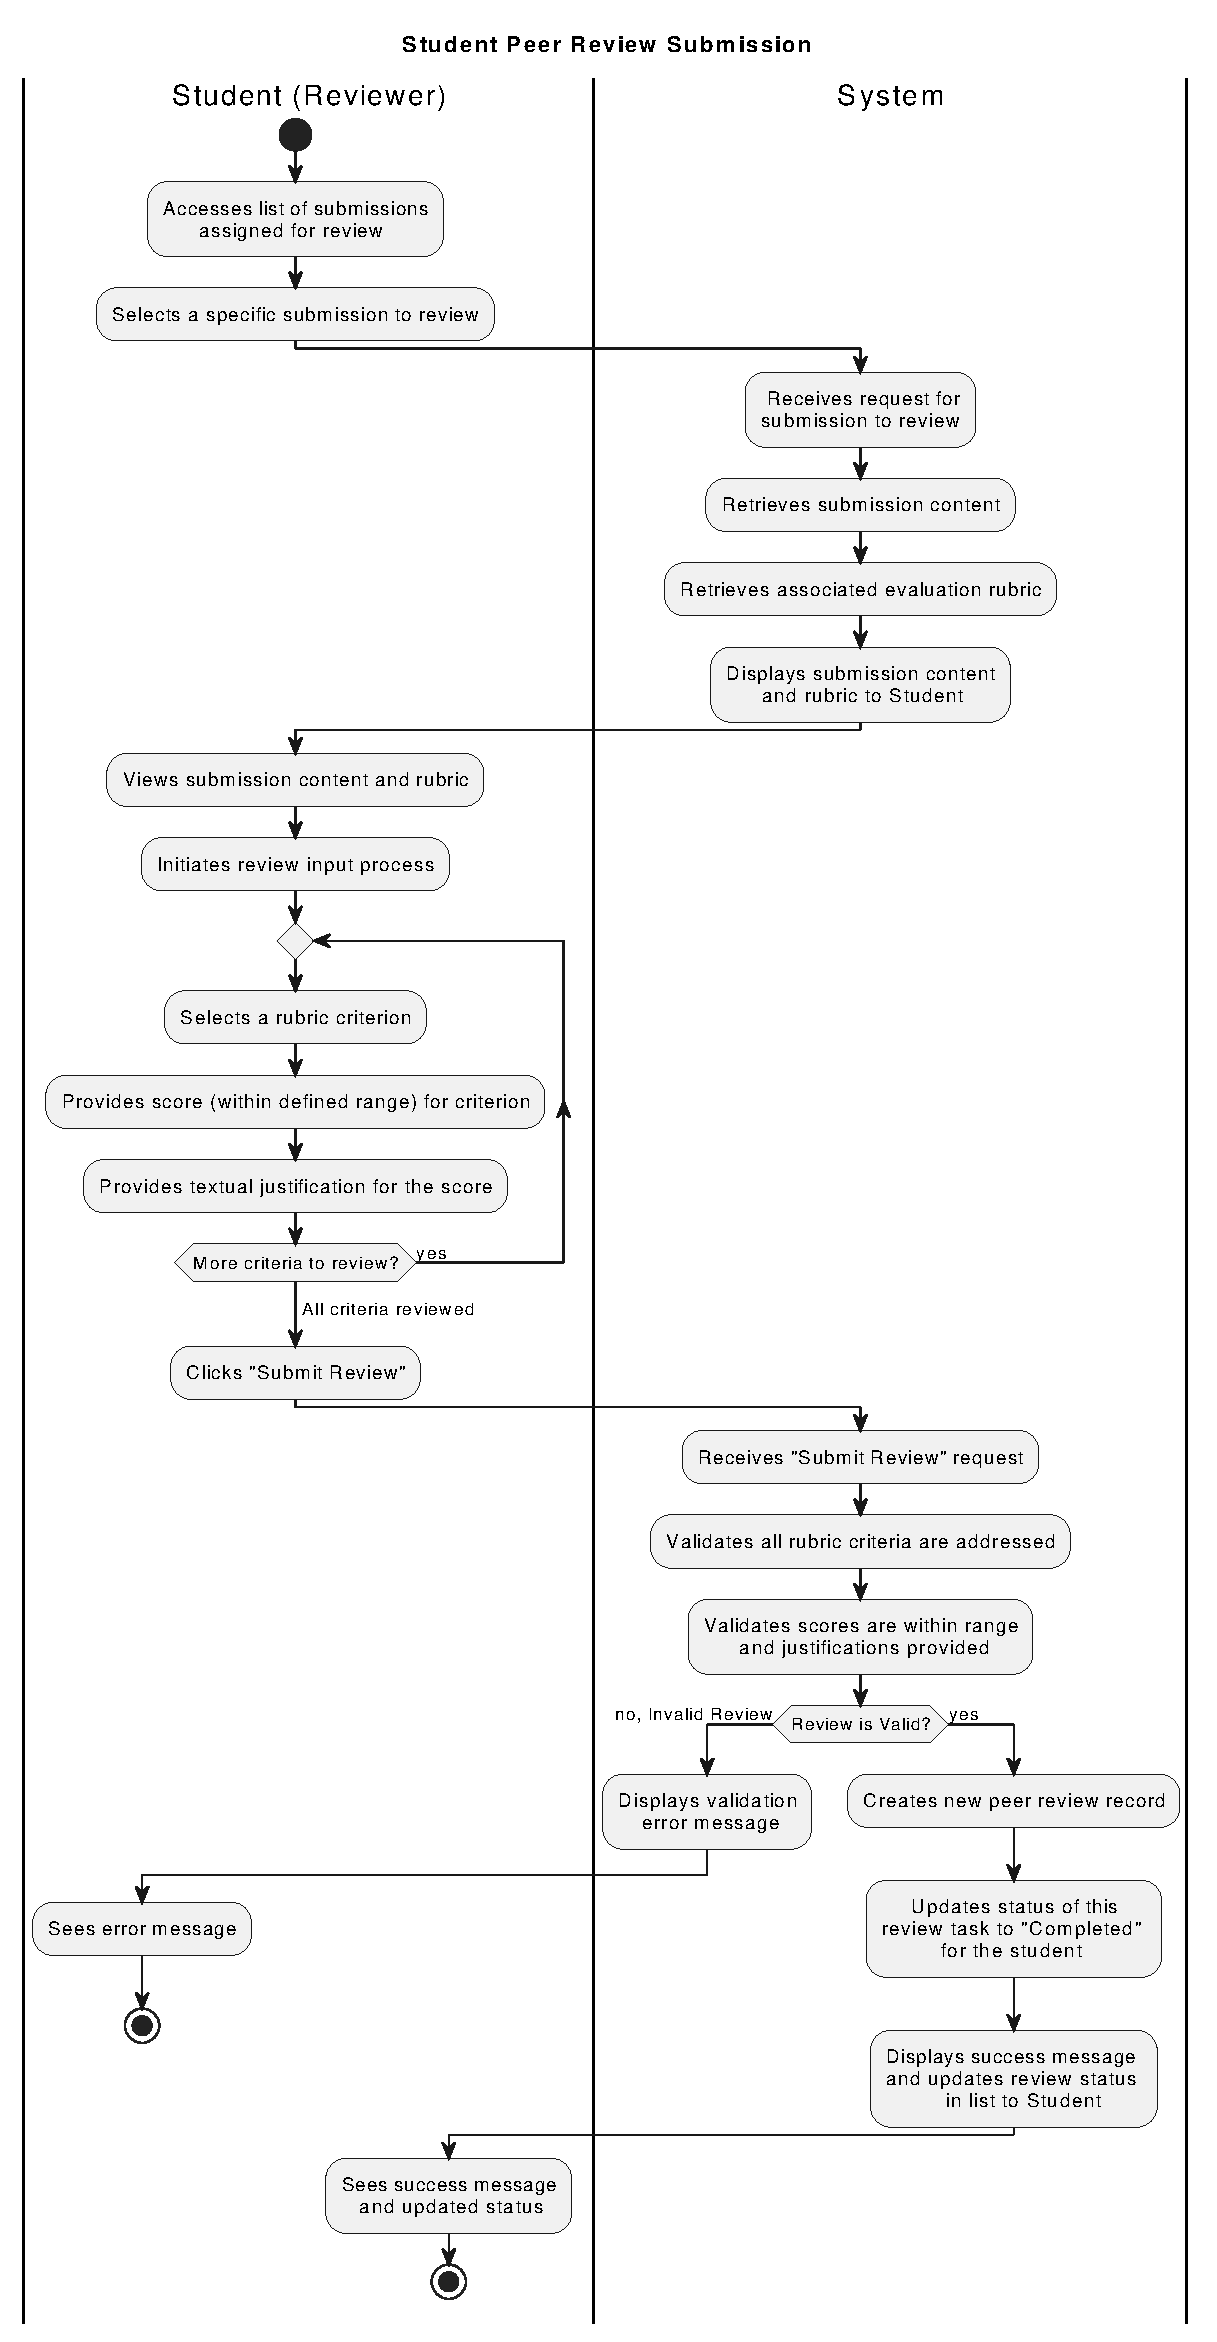
\includegraphics[width=.75\linewidth]{SRS/imgs/5_StudentPeerReviewCreation.pdf}
    \caption{Student Peer Review Submission Activity Diagram.}
    \label{fig:StudentPeerReviewAD}
\end{figure}
\vspace*{\fill}
\clearpage

\vspace*{2cm}

\subsection{Results \& Monitoring - All Users}

\begin{longtable}{|l|c|p{10cm}|}
    \hline
    \textbf{ID} & \textbf{Priority} & \textbf{Requirement} \\
    \endhead % This marks the end of the table header
    \hline
    FR-RES-001 & M & The system shall enable authenticated Teachers to monitor the submission status for assignments, particularly when the assignment is in a stage where submissions are expected, or when the deadline is expired and the peer review process is not started yet (e.g., "assigned", "preparing review"). This includes viewing aggregate submission counts and details of individual student submissions. \\
    \quad FR-RES-001.UI &  & \quad The system's UI shall provide a dedicated section or view, accessible to authenticated Teachers, when the assignment status is “assigned” or “preparing review” (prior to peer review distribution). The UI shall display the total number of students assigned to the assignment, the number of students who have submitted their work, and a list of submitted assignments, showing the student’s name, the submission status and a timestamp of the submission. \\
    \quad FR-RES-001.BL &  & \quad When an authenticated Teacher requests the detailed information of an assignment for which the peer review process is not started yet, the business logic shall retrieve the list of all students assigned to participate in this assignment, and determine their submission status by checking for a corresponding submission record; if it exists, retrieve the submission timestamp. The business logic shall calculate the aggregate statistics (total assigned, total submitted) as required by FR-RES-001.UI, and return them to the view. \\
    \hline
\end{longtable}

\begin{table}[h]
    \centering
    \caption{Results \& Monitoring Functional Requirements (1).}
    \label{tab:ResultMonitoringFR1}
\end{table}

\clearpage
\vspace*{1cm}

\begin{longtable}{|l|c|p{10cm}|}
    \hline
    \textbf{ID} & \textbf{Priority} & \textbf{Requirement} \\
    \endhead % This marks the end of the table header
    \hline
    FR-RES-002 & M & The system shall enable authenticated Teachers to monitor the progress of peer reviews for assignments, specifically when the assignment is in the "Under Review" stage. This includes viewing aggregate review completion statistics and detailed progress for individual reviewers and submissions. \\
    \quad FR-RES-002.UI &  & \quad When an assignment is in the "Peer Review" stage, the system's UI shall provide a dedicated section or view, showing the total number of expected peer reviews, number of peer reviews completed, total number of submissions requiring peer review, number of submissions for which all assigned peer reviews have been completed. The UI shall display a detailed list of all students assigned as reviewers for this assignment. For each reviewer, the list shall indicate the reviewers name or identifier, number of reviews assigned to them and number of reviews they have completed. The UI may provide an option to view a more detailed breakdown per submission, showing which reviewers are assigned to it and the status of each of those specific reviews. \\
    \quad FR-RES-002.BL &  & \quad Upon a request from an authenticated Teacher to monitor the peer review progress for a specific assignment (and which is in the "Under Review" stage), the business logic shall retrieve all peer review allocation records for the assignment (i.e., which student is assigned to review which submission) and calculate the aggregate statistics based on the status of the peer reviews. The business logic shall also calculate for each submission how many assigned reviews it has received and how many are completed. The business logic shall aggregate data for each reviewer, calculating the total reviews assigned to them and the number they have completed. Finally, the necessary data shall be returned to the view. \\
    \hline
\end{longtable}
\begin{table}[h]
    \centering
    \caption{Results \& Monitoring Functional Requirements (2).}
    \label{tab:ResultMonitoringFR2}
\end{table}
\clearpage

\begin{longtable}{|l|c|p{10cm}|}
    \hline
    \textbf{ID} & \textbf{Priority} & \textbf{Requirement} \\
    \endhead % This marks the end of the table header
    \hline
    FR-RES-003 & M & The system shall, after the peer review period for an assignment is completed, aggregate evaluation results and enable authenticated Teachers to view both overall assignment statistics (e.g., average scores per criterion, score distributions) and detailed reports for each individual student's submission, including the original submission content and all peer reviews received (scores, justifications, and reviewer identities). \\
    \quad FR-RES-003.UI &  & \quad Once the peer review period for an assignment created by an authenticated Teacher is completed (“Completed” state), the system's UI shall provide a dedicated section or view for accessing peer review results. It shall show aggregated statistics for the entire assignment, including the average score for each criterion in the rubric, score distribution visualizations and the overall average or aggregated score. Alongside the overall results view, the UI shall display a list of all student submissions for the assignment. It shall include for each submission the name of the student who authored it, the number of peer reviews completed for this submission versus the number assigned, an aggregated or average score for the single submission, and a button to access a detailed report view. This view shall include the original submitted text content and associated files, and a section for each peer review received by the submission, including the name of the student who performed the review and score and explanation for each criterion in the rubric. The UI shall provide clear navigation to return from the detailed submission report view back to the overall assignment results view or the submission list. \\
    \quad FR-RES-003.BL &  & \quad Upon a request from an authenticated Teacher to view peer review results for a specific assignment they created, The business logic shall retrieve all completed peer review records associated with all submissions for that assignment (including scores and explanations). For each criterion in the assignment's rubric, the business logic shall calculate the average score across all reviews for all submissions, and the distribution of scores, and finally return this data to the view. For the submission list and detailed report view, the business logic shall retrieve the list of all original submissions for the assignment, along with the identity of the student author for each, and associate the submission to its reviews. 
    \hline
\end{longtable}
\clearpage
\begin{longtable}{|l|c|p{10cm}|}
    \hline
    \textbf{ID} & \textbf{Priority} & \textbf{Requirement} \\
    \endhead % This marks the end of the table header
    \hline
     & & When a Teacher requests the detailed report for a specific submission, the business logic shall retrieve the content of the submission, and the data associated with each review, including the name of the student who performed that review, and finally return all this data to the view. \\
    \hline
    FR-RES-004 & M & The system shall allow Students to view the aggregated evaluations and motivated feedback they received on their own submissions, after the review process is completed and results are released. \\
    \quad FR-RES-004.UI &  & \quad Once peer review results for an assignment are officially released, the system's UI shall provide a dedicated section or view for an authenticated Student to access the feedback received on their submission for that assignment. This initial view for their submission shall display the student’s own submitted work, average score for each criterion in the rubric, and an average or aggregated score for their submission. The UI shall also display a list of all the individual peer reviews, including the name of the reviewer, and average or aggregated score given in that specific review. Upon selecting a review from the list, a new view shall display for each criterion the score and explanation. The UI shall provide clear navigation to return from the detailed individual review view back to the summary feedback view or the list of reviews. \\
    \quad FR-RES-004.BL &  & \quad Upon a request from an authenticated Student to view feedback received on their submission for a specific assignment (for which results have been released), the business logic shall retrieve all completed peer review records associated with the Student's specific submission for that assignment, and the Student's original submission content (text and file references). The business logic shall calculate an overall average or final aggregated score for the Student's submission based on a predefined aggregation method. For each peer review record retrieved (in 1.b), the business logic shall prepare the data for display, including: the identity (e.g., name) of the Student who performed the review, the scores and textual justifications provided for each criterion by that reviewer. \\
    \hline
\end{longtable}

\begin{table}[h]
    \centering
    \caption{Results \& Monitoring Functional Requirements (3-4).}
    \label{tab:ResultMonitoringFR3}
\end{table}

\clearpage

\begin{figure}[h]
    \centering
    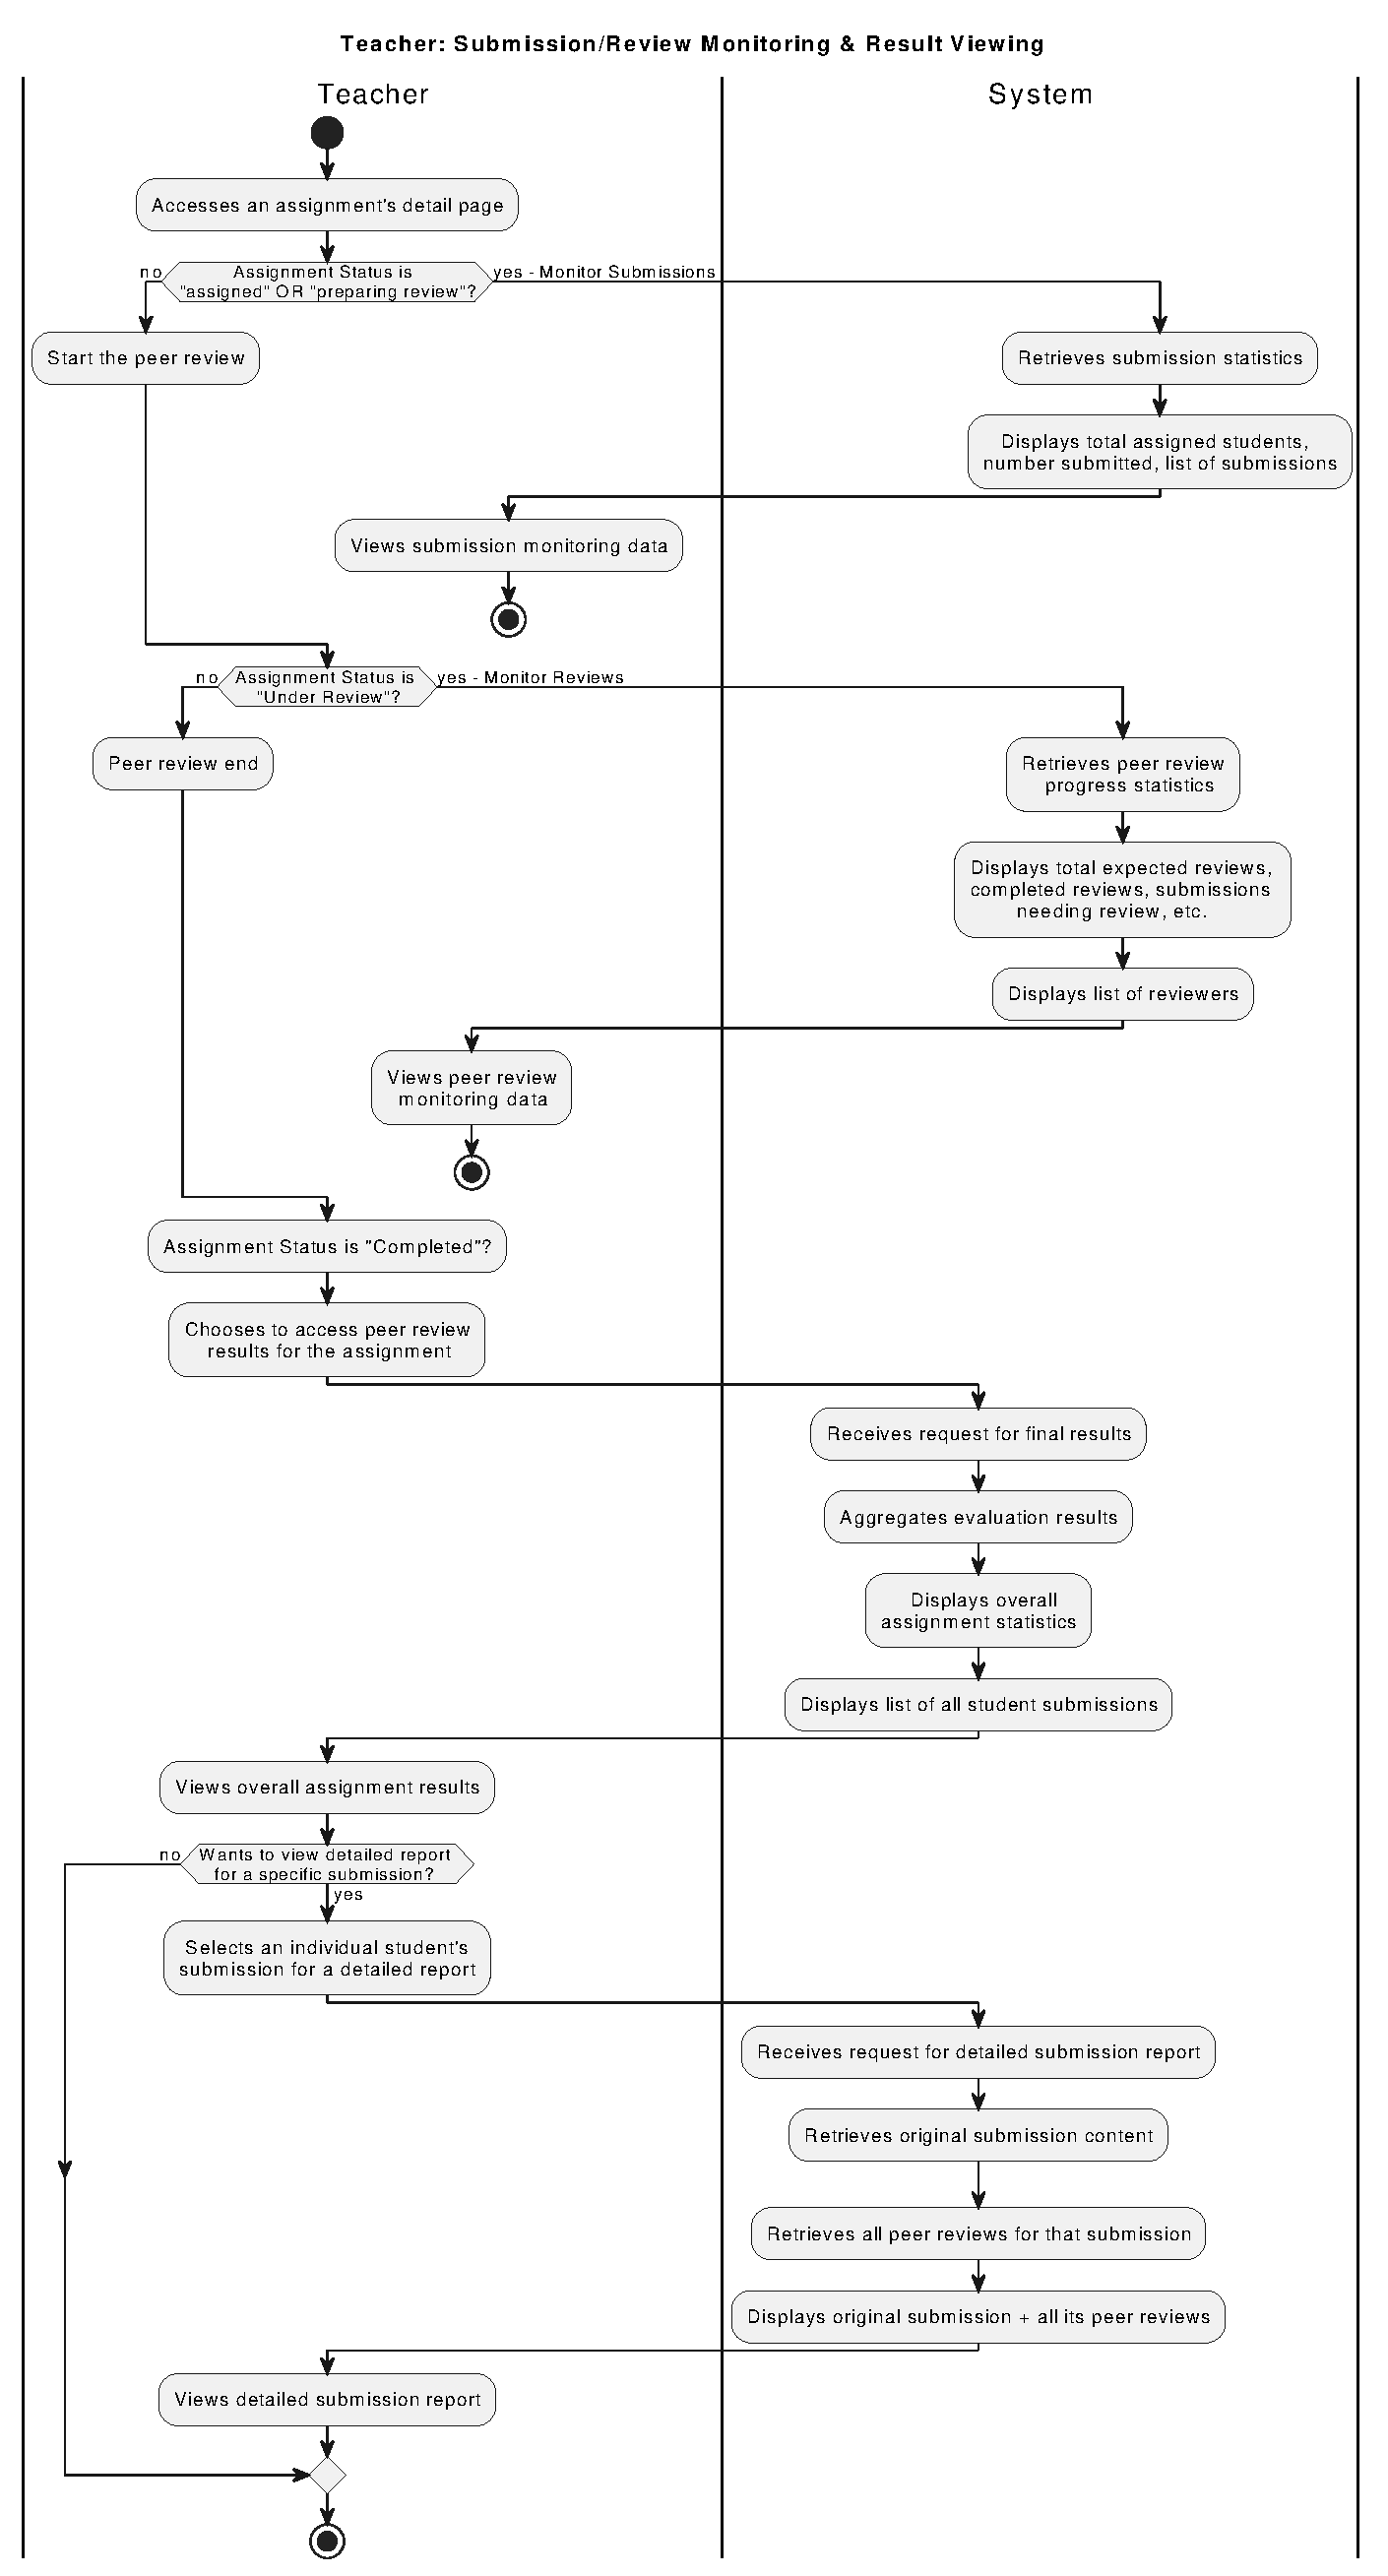
\includegraphics[width=0.7\linewidth]{SRS/imgs/6_TeacherMonitoring.pdf}
    \caption{Teacher Monitoring Review Activity Diagram.}
    \label{fig:TeacherMonitoringAD}
\end{figure}

\clearpage

\begin{figure}[h]
    \centering
    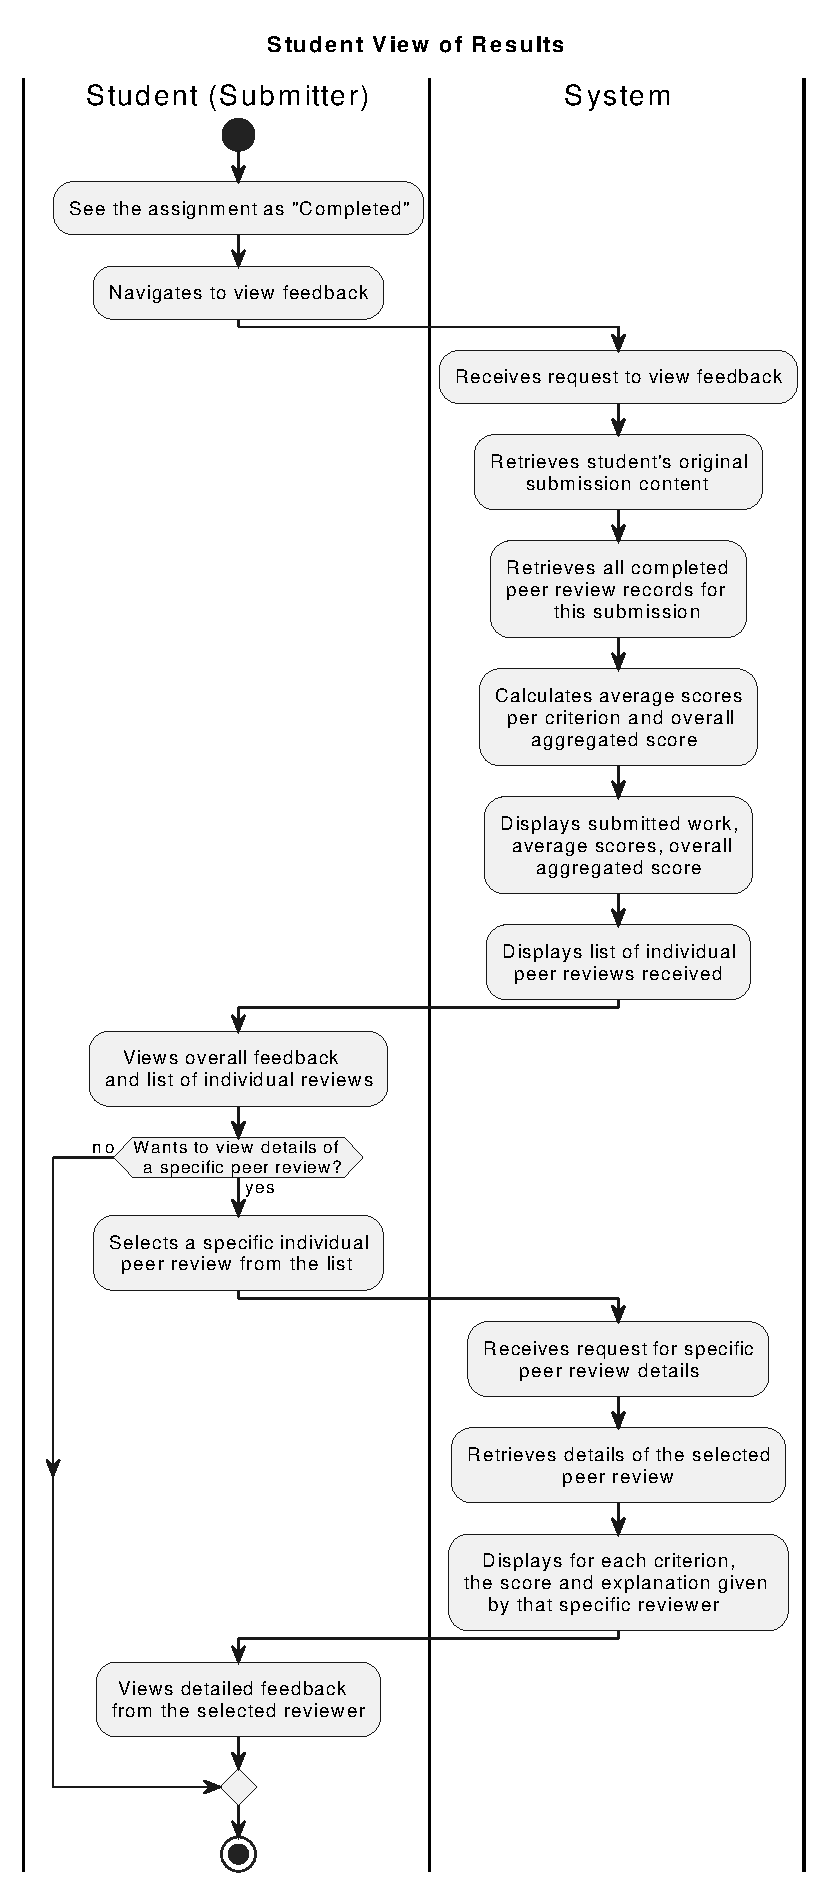
\includegraphics[width=0.6\linewidth]{SRS/imgs/7_StudentResult.pdf}
    \caption{Students Receive Results Activity Diagram.}
    \label{fig:StudentsResultsAD}
\end{figure}

\clearpage

\vspace*{1cm}

\subsection{Use Case Diagram}

\begin{figure}[h]
    \centering
    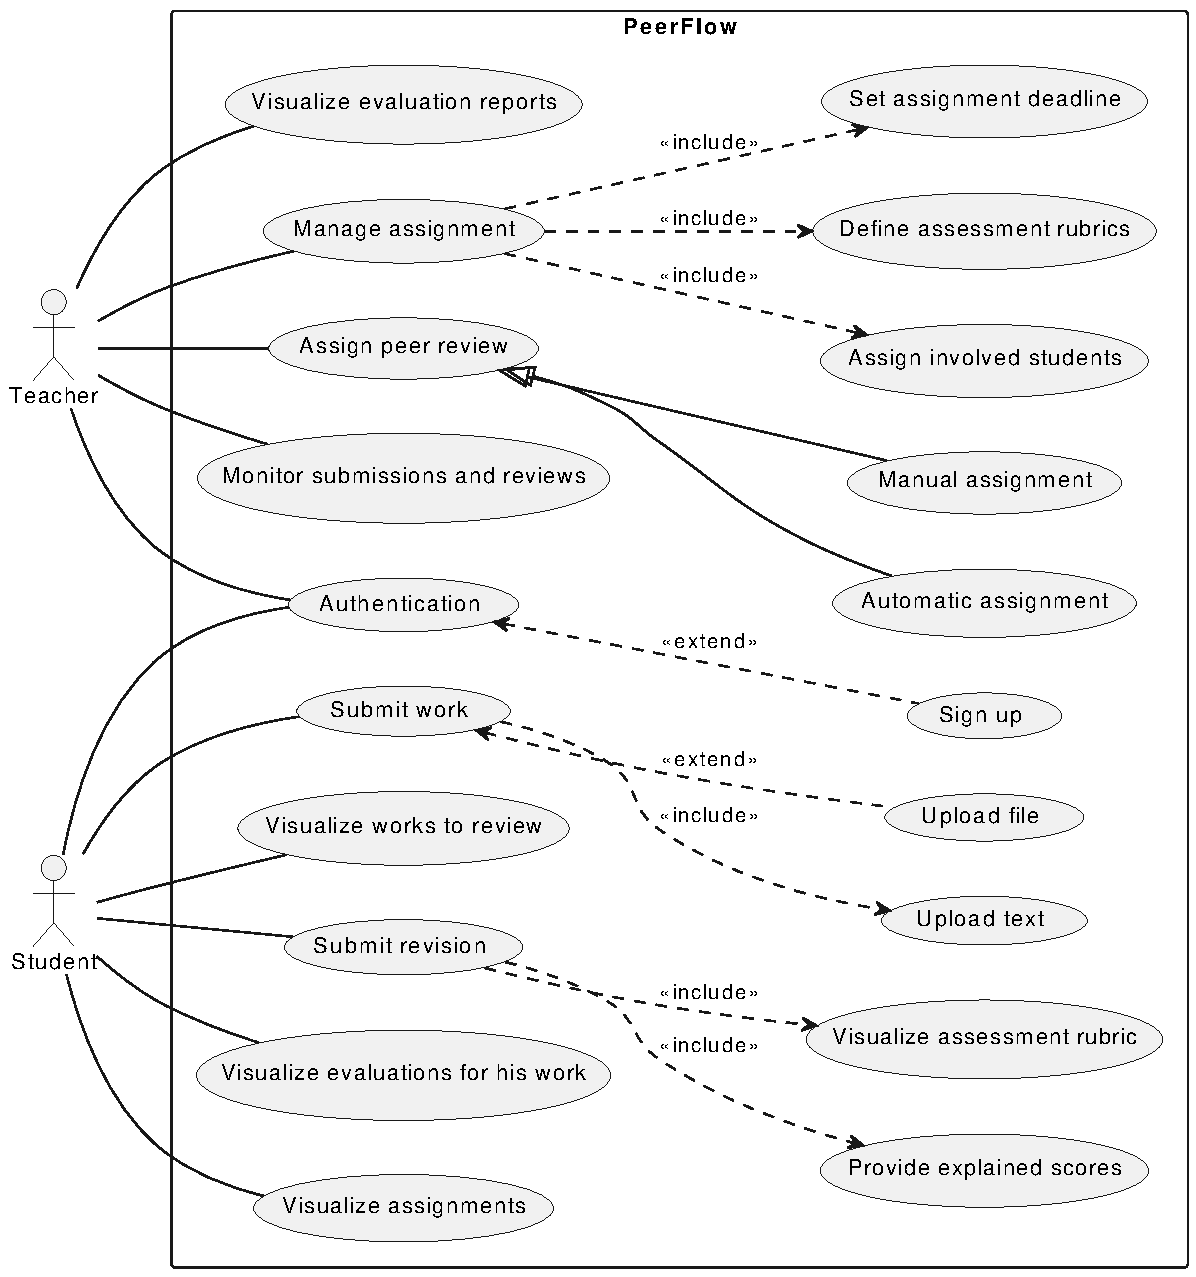
\includegraphics[width=0.9\linewidth]{SRS/imgs/GeneralUseCase.pdf}
    \caption{Complete Use Case Diagram}
    \label{fig:GeneralUseCase}
\end{figure}

\clearpage

\section{Non Functional Requirements}

\begin{justify}
    This subsection specifies the quality attributes that the PeerFlow system must exhibit. Unlike functional requirements that describe what the system does, non-functional requirements describe how well the system performs its functions. These attributes are critical for the overall success and user satisfaction of a MOOC-like platform.
    The quality attribute requirements will be specified using QA Scenarios:
    \begin{enumerate}
        \item \textbf{Source of Stimulus}: some entity (a human, a computer system, etc.) that generated the stimulus.
        \item \textbf{Stimulus}: an event that requires a response by the system.
        \item \textbf{Artifact}: the part of the system that is stimulated (may be the whole system).
        \item \textbf{Environment}: the circumstances in which the scenario takes place (system in normal state, overloaded, shutting down, ...).
        \item \textbf{Response}: the activity undertaken by the system (for runtime QA) or by developers (for dev. QA) as the result of the stimulus.
        \item \textbf{Response Measure}:  how to measure whether the response is satisfactory.
    \end{enumerate}
\end{justify}

\subsection{Modifiability}

\begin{comment}
    \begin{justify}
        This section describes the requirements that ensure PeerFlow can be easily modified, updated, and extended in the future. It focuses on aspects that facilitate the system's long-term evolution and support.
    \end{justify}
\end{comment}


\subsubsection{Scenario QA-MO-01: Modifying the Student Data Model}
\begin{itemize}
    \item \textbf{Source:} Developer.
    \item \textbf{Stimulus:} The project team decides to add a new mandatory field (e.g., "Student ID Number") to the student data model, requiring updates to the registration form and database query logic.
    \item \textbf{Artifact:} The Authentication and Profiling microservice (for user profile and registration) and potentially other services interacting with student data (e.g., Course Management, Assignment Management).
    \item \textbf{Environment:} The system is in the Development environment.
    \item \textbf{Response:} The student data model is successfully updated, the registration form is modified to include the new field, and all database queries for student information are adapted to handle the change without errors.
    \item \textbf{Response Measure:} The modification, including schema changes, form updates, and logic adjustments, is completed and unit-tested within 6 hours of effort, affecting a localized set of files within the relevant microservices.
\end{itemize}

\subsubsection{Scenario QA-MO-2: Adding a New Submission File Type}
\begin{itemize}
    \item \textbf{Source:} Product Owner.
    \item \textbf{Stimulus:} The product owner decides to allow students to submit an additional file type (e.g., .zip for code archives) for assignments.
    \item \textbf{Artifact:} The Assignment Management microservice, specifically the file submission and storage components.
    \item \textbf{Environment:} The system is in the Development environment.
    \item \textbf{Response:} The system successfully accepts and stores the new file type, and the UI displays it correctly.
    \item \textbf{Response Measure:} The change to support the new file type is made and tested within 4 hours.
\end{itemize}

\subsection{Integrability}

\subsubsection{Scenario QA-IN-1: Integrating a Basic Student Notification Service}
\begin{itemize}
    \item \textbf{Source:} Mission/system stakeholder.
    \item \textbf{Stimulus:} The project team decides to integrate a new, dedicated notification service to send basic email or in-app notifications to students regarding new assignment availability and peer review assignments.
    \item \textbf{Artifact:} The Assignment Management and Peer Review Management microservices (as triggers) and a new Notification microservice (as the provider of the notification functionality).
    \item \textbf{Environment:} The system is in the Development environment.
    \item \textbf{Response:} The Assignment Management and Peer Review Management services successfully trigger notifications via the new Notification service, and students receive timely and accurate alerts.
    \item \textbf{Response Measure:} The integration, including defining and implementing the Notification service's API, and modifying the triggering services, is completed and end-to-end tested within 8 hours, with notification delivery verified for correctness.
\end{itemize}

\subsubsection{Scenario QA-IN-2: Enabling a Basic Health Check Endpoint for Service Discovery}
\begin{itemize}
    \item \textbf{Source:} Developers.
    \item \textbf{Stimulus:} A requirement arises to expose a basic health check endpoint for each microservice to facilitate automated service discovery and monitoring within the Kubernetes cluster.
    \item \textbf{Artifact:} All existing microservices, requiring the addition of a simple HTTP endpoint.
    \item \textbf{Environment:} The system is in the Development environment or Integration environment.
    \item \textbf{Response:} Each microservice provides a functional /health endpoint that returns a successful status (e.g., HTTP 200 OK), allowing Kubernetes to correctly determine service availability.
    \item \textbf{Response Measure:} The implementation of the health check endpoint for all microservices is completed and verified within 4 hours, requiring only the addition of a basic endpoint and no complex logic.
\end{itemize}

\subsection{Deployability}

\subsubsection{Scenario QA-DE-1: Rolling Back a Malfunctioning Peer Review Management Service}
\begin{itemize}
    \item \textbf{Source:} System administrator.
    \item \textbf{Stimulus:} A newly deployed version of the Peer Review Management microservice exhibits unexpected behavior and high latency in the production environment.
    \item \textbf{Artifact:} The Peer Review Management microservice.
    \item \textbf{Environment:} The Production environment.
    \item \textbf{Response:} The system is rolled back to the previous stable version of the Peer Review Management service, and normal operation is restored.
    \item \textbf{Response Measure:} The rollback is initiated and completed within 10 minutes, with no data loss or negative impact on other services.
\end{itemize}

\subsection{Availability}

\subsubsection{Scenario QA-AV-1: Service Instance Failure}
\begin{itemize}
    \item \textbf{Stimulus Source:} Unexpected failure (e.g., process crash, hardware issue on the VM) of a Review Service instance.
    \item \textbf{Stimulus:} The service instance stops responding to requests.
    \item \textbf{Artifact:} The Review Service.
    \item \textbf{Environment:} Normal operation, during student review processing.
    \item \textbf{Response:} The orchestrator detects the instance failure and automatically redirects traffic to healthy instances. A new instance is launched to replace the failed one.
    \item \textbf{Response Measure:}
    \begin{itemize}
        \item Failover to a healthy instance occurs within 30 seconds of failure detection.
        \item Users in session who were interacting with the failed instance might experience a single error, but subsequent attempts are successful.
        %\item Overall service availability remains $\ge 99.95\%$ on a monthly basis.
    \end{itemize}
\end{itemize}

\subsection{Performance}

\subsubsection{Scenario QA-PE-1: Assignment Page Loading}
\begin{itemize}
    \item \textbf{Stimulus Source:} A student clicks to view the details of an assignment.
    \item \textbf{Stimulus:} HTTP GET request for the assignment description page, which includes rubrics and attachments.
    \item \textbf{Artifact:} The User Interface and the Assignment Service.
    \item \textbf{Environment:} Normal operation, with an average load of 50,000 concurrent users.
    \item \textbf{Response:} The system retrieves assignment information, rubrics, and attachment metadata, and renders the page in the student's browser.
    \item \textbf{Response Measure:}
    \begin{itemize}
        \item Server-side response time (Time To First Byte - TTFB) for assignment data is less than 300 ms for the 95th percentile of users.
        \item Total page load time (Largest Contentful Paint - LCP) is less than 2.5 seconds for the 75th percentile of users.
    \end{itemize}
\end{itemize}

\subsubsection{Scenario QA-PE-2: Saving a Review}
\begin{itemize}
    \item \textbf{Stimulus Source:} A student submitting a completed review for a peer's assignment.
    \item \textbf{Stimulus:} HTTP POST request containing review data (text, scores according to rubric).
    \item \textbf{Artifact:} The User Interface and the Review Service.
    \item \textbf{Environment:} Normal operation, peak review activity (e.g., day before review deadline).
    \item \textbf{Response:} The system validates and saves the review data in the database and confirms the operation to the student.
    \item \textbf{Response Measure:}
    \begin{itemize}
        \item The processing time for the save request and confirmation to the user is less than 1 second for the 90th percentile of users.
        \item In case of failed validation, feedback is provided within 500 ms.
    \end{itemize}
\end{itemize}

\subsubsection{Scenario QA-PE-3 - Scalability: Submission Peak}
\begin{itemize}
    \item \textbf{Stimulus Source:} A large number of students (e.g., 100,000) attempting to submit their assignments concurrently.
    \item \textbf{Stimulus:} Multiple file submission requests (text and attachments) within the last 30 minutes before the deadline of a popular assignment.
    \item \textbf{Artifact:} The Assignment Service and the underlying storage infrastructure.
    \item \textbf{Environment:} Normal operation, but during a projected peak load period.
    \item \textbf{Response:} The system accepts all submissions without errors, horizontally scaling Assignment Service instances and necessary storage resources to handle the load.
    \item \textbf{Response Measure:}
    \begin{itemize}
        \item All submission requests are successfully processed within 1 minute of reception.
        \item The error rate for submissions remains below $0.01\%$.
    \end{itemize}
\end{itemize}

\clearpage

\subsubsection{Scenario QA-PE-4 - Scalability: Increase in Registered Users}
\begin{itemize}
    \item \textbf{Stimulus Source:} The registration of 1 million new users to the MOOC platform over a week following a promotional campaign.
    \item \textbf{Stimulus:} Gradual but significant increase in the number of active users, profile creation requests, and general platform interactions (assignment viewing, etc.).
    \item \textbf{Artifact:} All services, with particular emphasis on the Authentication Service and Assignment Service.
    \item \textbf{Environment:} Normal operation, with a trend of increasing load.
    \item \textbf{Response:} The system handles the increased number of users and their activities while maintaining performance and availability levels, scaling resources transparently.
    \item \textbf{Response Measure:}
    \begin{itemize}
        \item Average response time for login remains less than 2 seconds.
        \item Average response time for viewing assignment information remains less than 2 seconds.
        \item The platform supports a $50\%$ increase in concurrent users (from 500,000 to 750,000) without degradation of key performance metrics, with a proportional increase in resources (not exceeding a $60\%$ increase).
    \end{itemize}
\end{itemize}

\subsection{Testability}

\subsubsection{Scenario QA-TE-1: Unit Test Coverage}
\begin{itemize}
    \item \textbf{Stimulus Source:} Developers, QA
    \item \textbf{Stimulus:} A new feature is integrated or an existing code section is modified.
    \item \textbf{Artifact:} The affected code module(s).
    \item \textbf{Environment:} Development.
    \item \textbf{Response:} The execution of unit tests must achieve a specified percentage of line code coverage, calculated using a standard code coverage tool.
    \item \textbf{Response Measure:} The overall line code coverage for unit tests must be equal to or greater than 80\%.
\end{itemize}
